\chapter[Concept]{Concept: Package Design, Theorema Integration, TeXForm Consideration – In Any Case Pattern-Matching-Based Expression Processing}
\label{cha:Concept}

Having already taken a broad conceptual introductory approach and weighed the relevant theory, it should be efficient to derive the concept for a program package dealing with transformation of the notebook format to \LaTeX at this point: The aim is to apply the strengths of WL as a programming language as directly as possible.

\section{Conceptual Cornerstones for this Project}

\subsection{WL-Native Approach for Direct Integration with Theorema}

The design for the package is such that it is intended to be integrated with the Theorema project as a stand-alone package. Figure \ref{fig:hierary} illustrates the relationship of this package to Theorema (Language) and Wolfram Language, as a whole.

\begin{figure}[h]
    \centering
    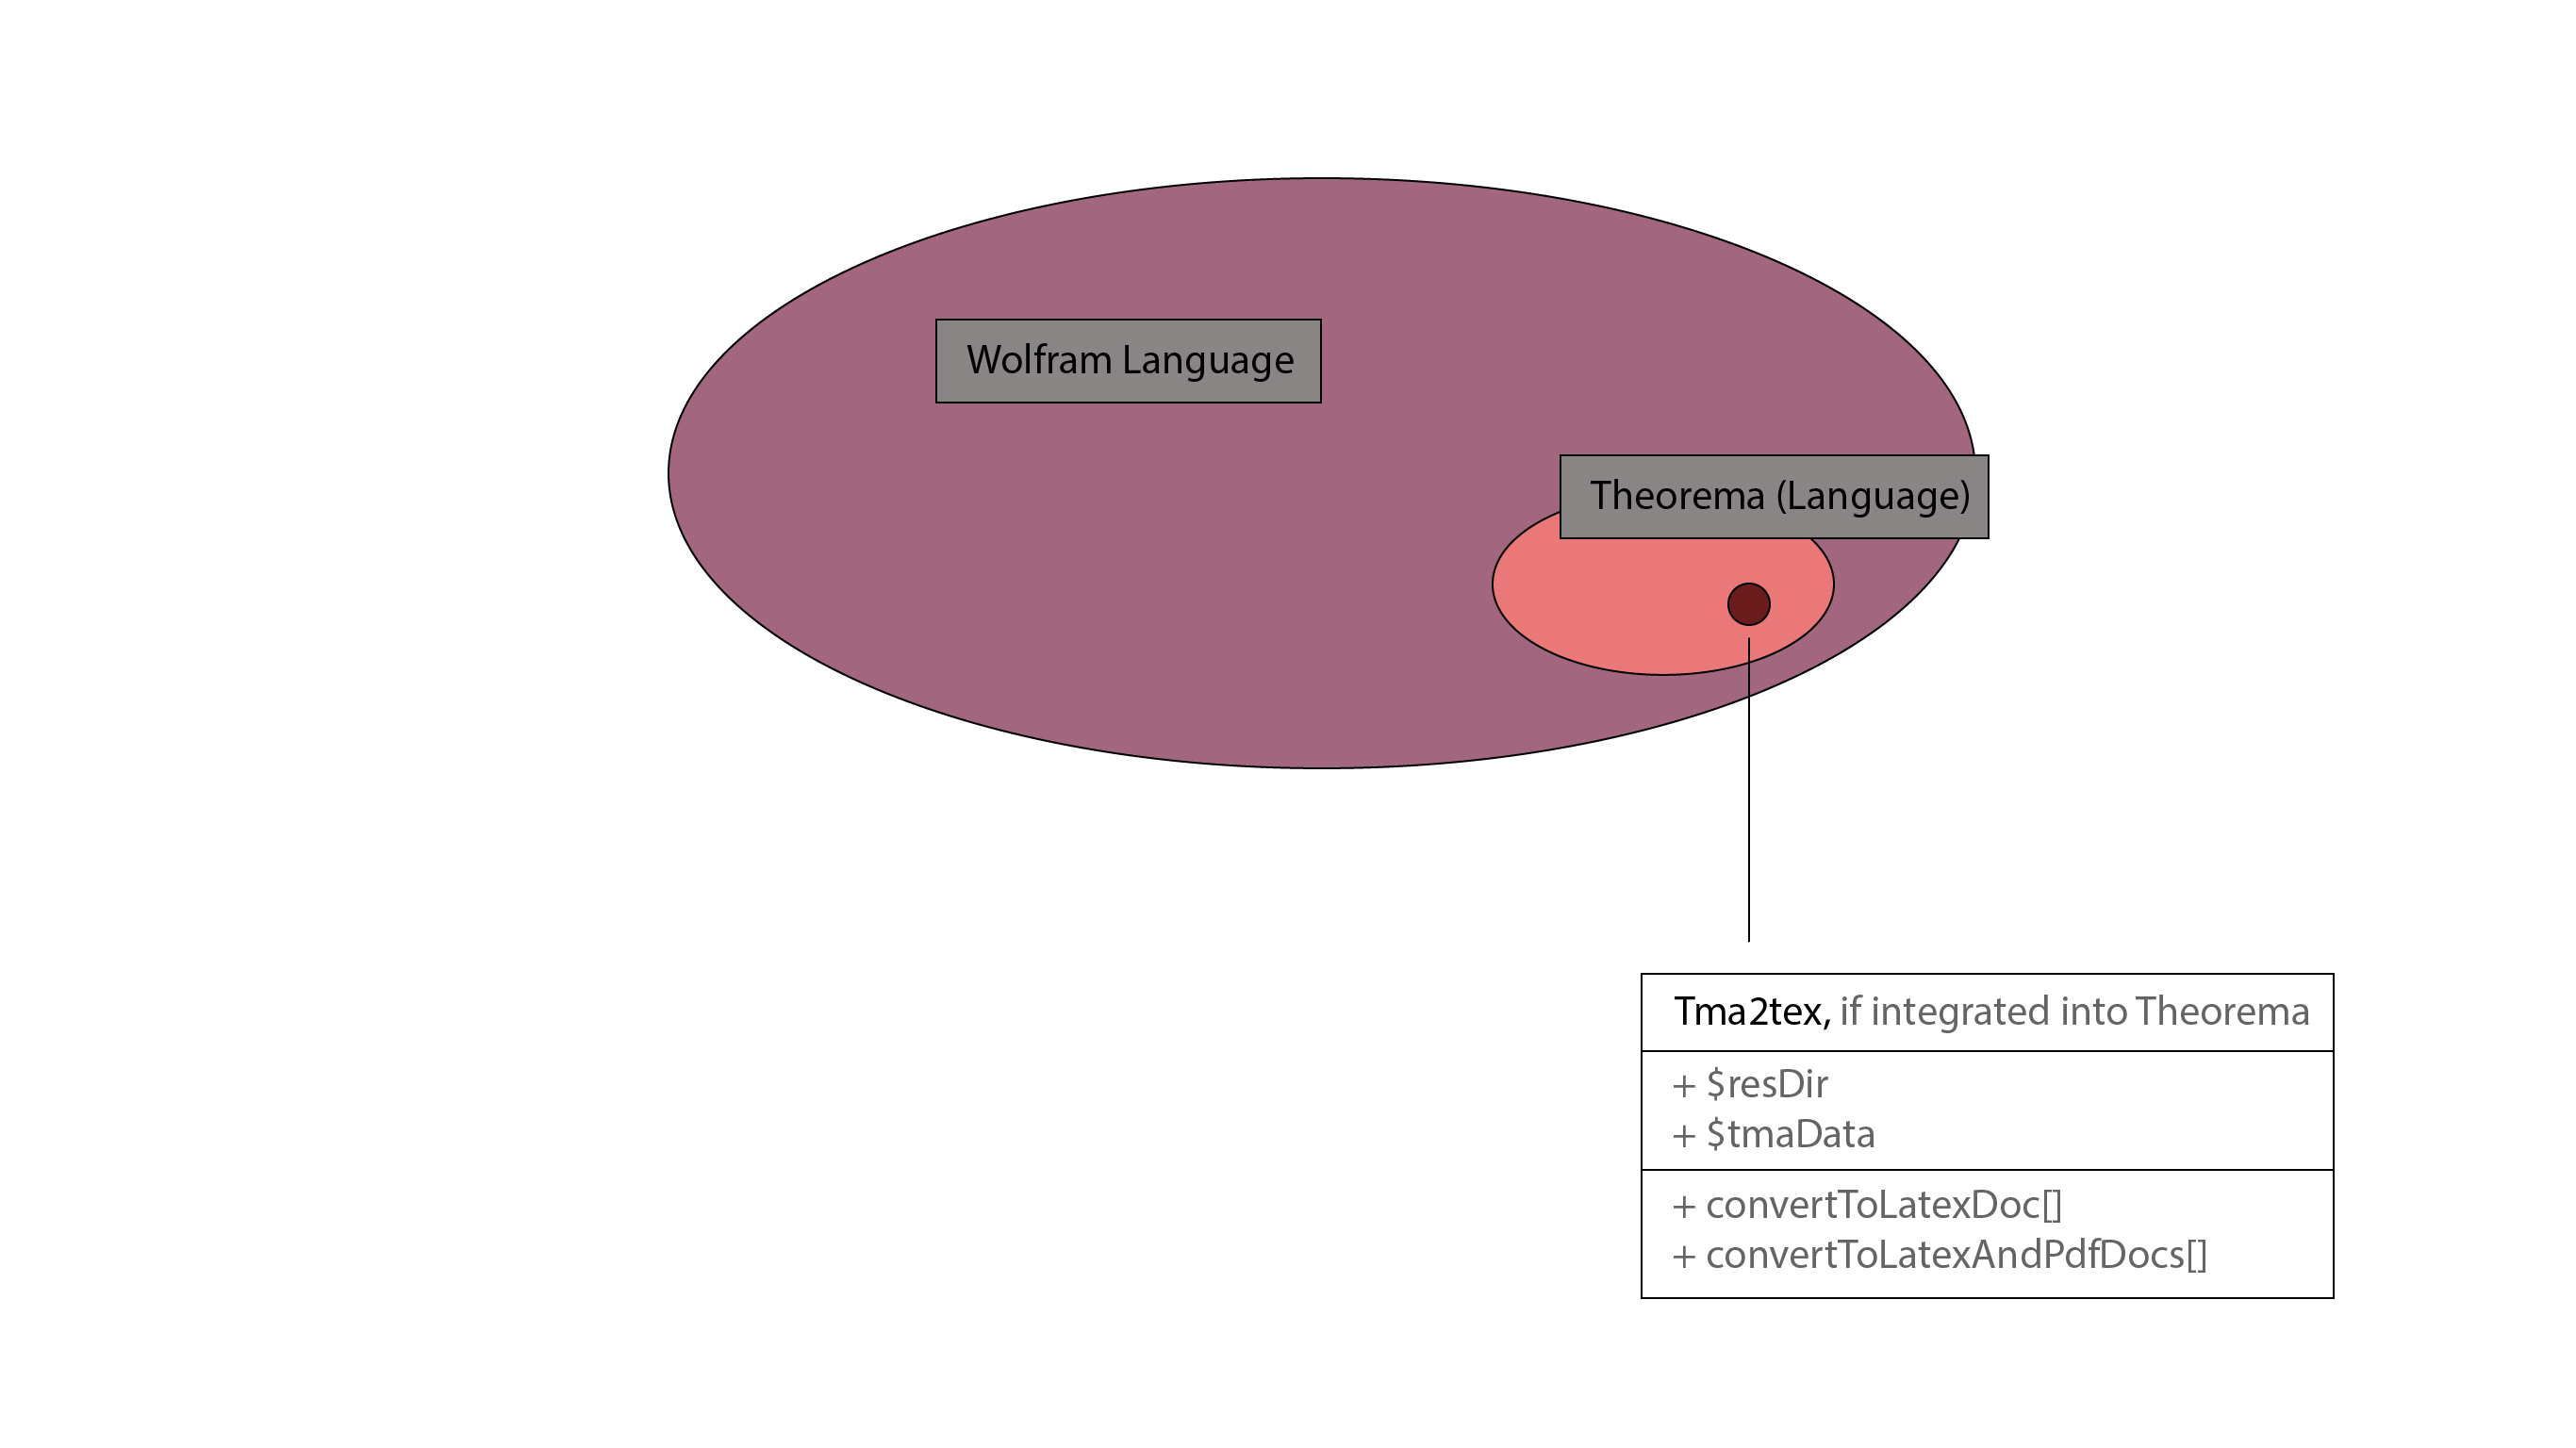
\includegraphics[scale=.35]{images/concept/Tma2Tex-Hierarchy.png}
    \caption{}
    \label{fig:hierary}
\end{figure}

The package itself is designed to follow the logic illustrated in Figure \ref{fig:package-logic}: files involved are colored green, code blue, transformation logic red - these are all the subject of this chapter.

\begin{figure}[h]
    \centering
    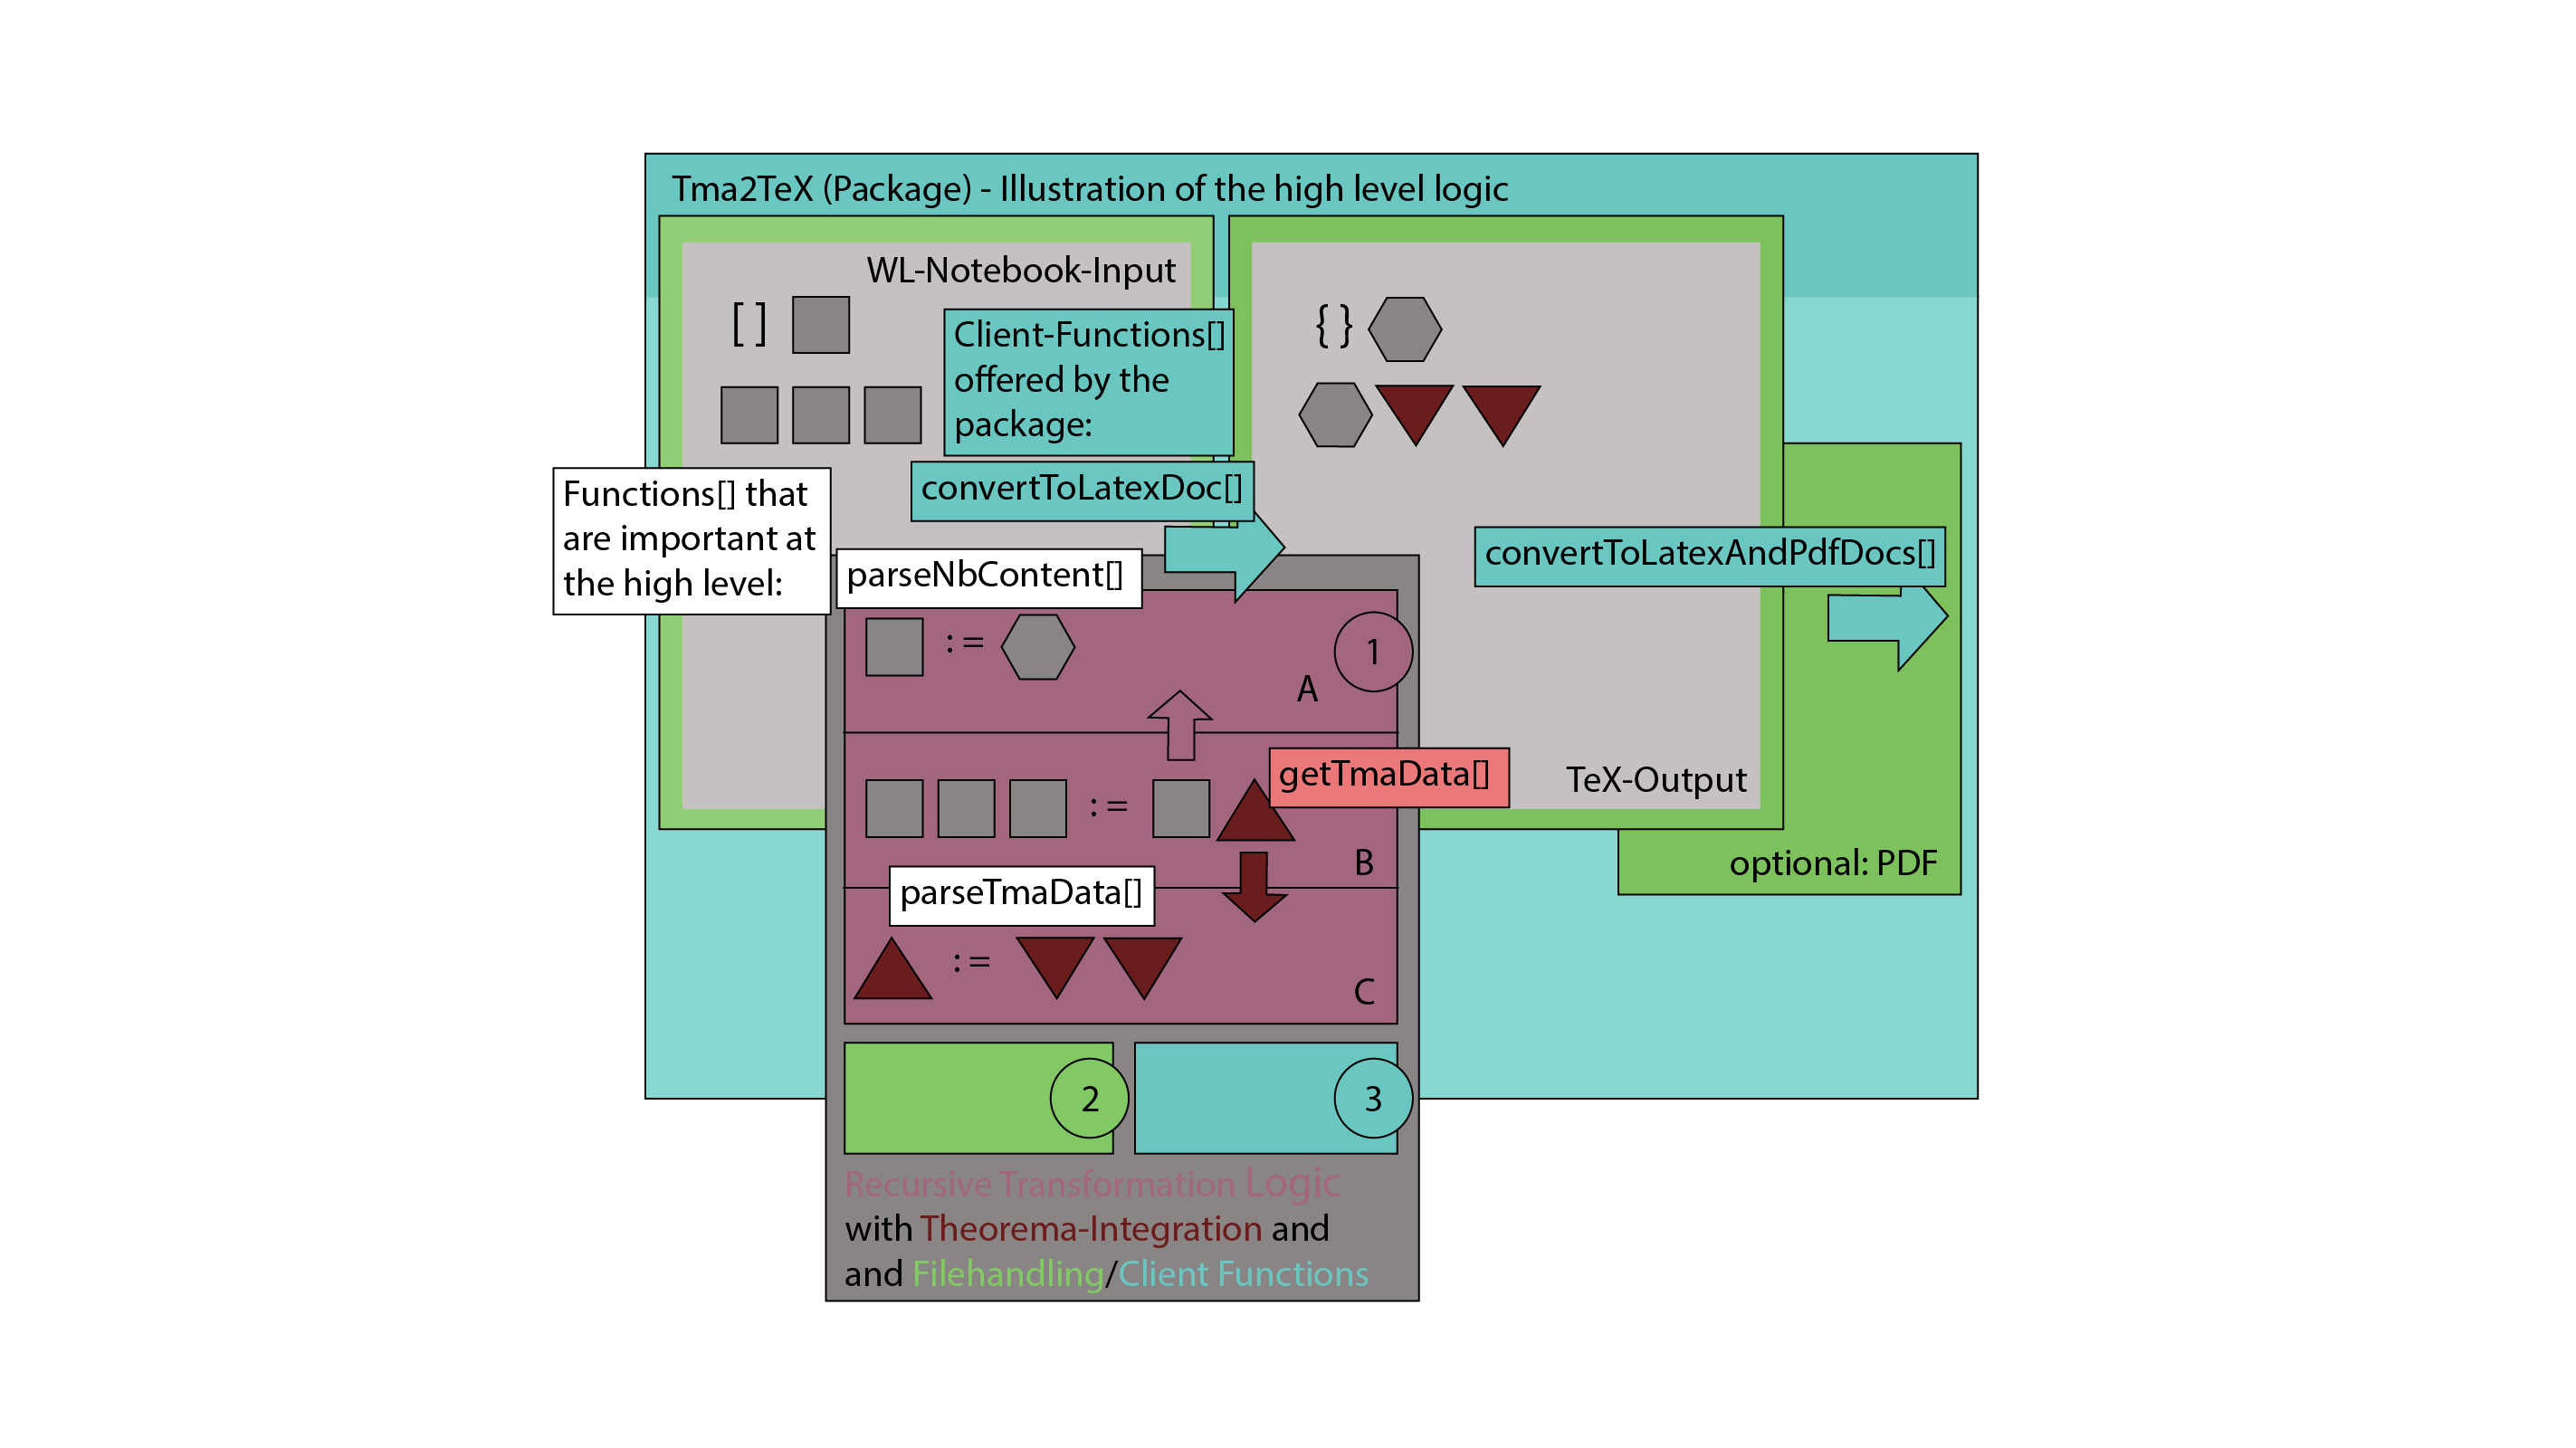
\includegraphics[scale=.35]{images/concept/Tma2Tex-Logic-01.png}
    \caption{}
    \label{fig:package-logic}
\end{figure}

This setup lends itself to an approach where the \LaTeX-template is used for customizations, at output: the template is filled by the \LaTeX generated by transforming the relevant Theorema Language formulas, particularly, but the Wolfram Language notebook as a whole, generally.

\subsection{Existing (Kernel) Functionality: Source Code Deep-Dive} \label{concept:existing-functionality}

The kernel sits at the core of the WL system (in keeping with the term in operating systems) and is available as a stand-alone program as well: "A standalone kernel session normally reads input from a device (typically a keyboard or a WSTP \cite{wolfram_research_inc_wstp_2024} connection), evaluates the expression and prints the result to a device (typically a screen or a WSTP connection)." \cite{wolfram_research_inc_wolframkernelwolfram_2024} Therefor the kernel needs to contain the main functionality expected for the WL system (independently of the notebook environment). From a software development standpoint, the kernel repository is the place to find the implementation for any essential function that a package outside of the kernel might rely on.

For this project, the main kernel function of relevance is TeXForm, which takes a WL expression and transforms it to its typesetting correlate in \LaTeX. Looking directly at the implementation reveals that the expedient way to handle this transformation is to exhaustively list and maintain the transformation rules in the form of a WL association. In order, the following categories (with one example each) make up most of the currently about 2000 lines of code inside the TeXForm package.

\begin{center}
    \begin{tabular}{||c c c||} 
         \hline
         Variable & Category of Symbol & Replacement Rule Example \\ [0.5ex] 
         \hline
         \hline
         \lstinline+$GreekLetters+ & Greek Letters & \lstinline+"\[Alpha]" -> "\\alpha "+ \\ 
         \hline
         \lstinline+$CaligraphicLetters+ & Caligraphy & \lstinline+"\[ScriptA]" -> "\\mathit{a}"+ \\
         \hline
         \lstinline+$GothicLetters+ & Gothic & \lstinline+"\[GothicA]" -> "\\mathfrak{a}"+ \\
         \hline
         \lstinline+$DoubleStruckLetters+ & Double-struck/Emphasis & \lstinline+"\[DoubleStruckA]" -> "\\mathbf{a}"+ \\
         \hline
         \lstinline+$AccentedLetters+ & Accented Letters & \lstinline+"\[AGrave]" -> "\\text{\\ a}"+ \\ [1ex] 
         \hline
         \lstinline+$MiscellaneousSymbols+ & Miscellaneous Symbols & \lstinline+"\[ConstantC]" -> "c"+ \\ 
         \hline
         \lstinline+$Shapes+ & Shapes & \lstinline+"\[FilledSquare]" -> "\\blacksquare"+ \\
         \hline
         \lstinline+$TextualForms+ & Special Characters & \lstinline+"\[DotlessI]" -> "\\text{\\i}"+ \\
         \hline
         \lstinline+$Operators+ & Operators & \lstinline+"\[Times]" -> "\\times"+ \\
         \hline
         \lstinline+$RelationSymbols+ & Symbols for Various Relations & \lstinline+"\[NotEqual]" -> "\\neq"+ \\ [1ex] 
         \hline
         \lstinline+$Arrows+ & Arrow-Symbols & \lstinline+"\[LeftArrow]" -> "\\leftarrow"+ \\ [1ex] 
         \hline
         \lstinline+$Spaces+ & Space-Characters & \lstinline+"\[ThickSpace]" -> "\\thickspace"+ \\ 
         \hline
         \lstinline+$Others+ & Other (Mathematical) Symbols & \lstinline+"\[Conjugate]" -> "*"+ \\
         \hline
         \lstinline+$LeftTeXDelimiterReplacements+ & Left Delimiters & \lstinline+"(" -> {"("}+ \\
         \hline
         \lstinline+$RightTeXDelimiterReplacements+ & Right Delimiters & \lstinline+")" -> {")"}+ \\
         \hline
         \lstinline+$TeXDelimiterReplacements+ & \LaTeX-Delimiters & \lstinline+"\\" -> {"\\backslash "}+ \\
         \hline
         \lstinline+$BasicEscapes+ & Escaped Characters & \lstinline+"#" -> "\\#"+ \\
         \hline
         \lstinline+$ASCIIUnchanged+ & ASCII characters & Function \\
         \hline
    \end{tabular}
\end{center}

This tabulation gives an idea of the type of transformations that would need to occur and implies for this project: while a mapping of a Theorema Language to WL expressions is possible in some cases (in fact a straightforward task in cases where the transformation is removing the suffix \lstinline+$TM+ and if needed, the full context with Theorema reference), any Theorema-to-\LaTeX transformation would be limited to symbols available in WL, negating the need and use of Theorema Language. Specific as-is output using notebook-level \LaTeX-transformation via file-export was already shown to be lacking in section \ref{intro:existing-functionality}.

Further, the pattern-matching-based \lstinline+parseNbContent+ allows for exactly the parts of the notebook of interest to the relevant user group, making the overall idea for the project a bespoke Theorema-TeXForm at notebook-level, in terms of existing WL-functionality, sitting neatly somewhere between a solution that solves expression-level TeX-transformation and notebook-level export.

As far as WL-TeXForm is concerned, all replacements are grouped together in an exhaustive list of replacements:

\begin{verbatim}
$TeXReplacements = Join[
  $ASCIIUnchanged, $BasicEscapes, $TeXDelimiterReplacements,
  $GreekLetters, (*$GreekWords,*) $AccentedLetters, $Spaces,
  $CaligraphicLetters, $GothicLetters, $DoubleStruckLetters,
  $MiscellaneousSymbols, $Shapes, $TextualForms,
  $Operators, $RelationSymbols, $Arrows, $Others
]
\end{verbatim}

These \lstinline+TeXReplacements+ inform the actual parsing in TeXForm. As has been argued already, TeXForm needs to be expanded in some way to permit Theorema-language parsing. Now a problem arises, however, because it is not as straightforward as a simple case-by-case switching between TeXForm and TheoremaTeXForm, say.

The (closed) source code for the Kernel would need to be opened to intertwine Theorema-specific functionality with TeXForm-functionality. This is illustrated by the fact that TexForm needs the complete expression to operate on successfully (maintaining correct nesting) and would not be useful called on an independent part (at any level in the expression hierarchy) individually: so \lstinline+TeXForm[And[Or[a,b], Or[c,d]]]+ would yield \lstinline+(a\\lor b)\\land (c\\lor d)+ natively, but called on the Theorema-language correlate at the outer level, that is \lstinline+ExpressionToTeX[And$TM[Or[a, b], Or[c, d]]]+, gives \lstinline+\\text{And$TM}(a\\lor b,c\\lor d)+: The text-rendering of unrecognized symbols is a sensible default. Calling a Theorema-version of TeXForm on only the And\$TM-expression, however, is problematic, because the TeXForm, as implemented in texformdump.wl and provided in the project repo, is fundamentally recursive to handle nested expressions. Without access to the way the operative recursive function (MakeTeX as it turns out) is called, a native-only TeXForm-solution would not work to handle Theorema language expressions in the proposed method.

The MakeTeX/makeTeX distinction is significant because it realizes the separation between the caller package and \verb+Texformdump`+, the package. makeTeX is the driver of the recursion-parsing, but calls MakeTeX in turn, which is only defined exactly once inside this base package, suggesting its usage to the user, the caller package:

\begin{verbatim}
(* Only built-in rule *)
MakeTeX[boxes_] := maketex[boxes]
\end{verbatim} 

Any overloading of MakeTeX overrides all corresponding maketex rules, so while it is important that maketex recursively calls MakeTeX, not maketex, maketex is doing the heavy lifting, and MakeTeX allows the user to override definitions at any expression level. MakeTeX-rules can also be defined inside the caller package in this way and it is by this mechanism that this project realizes the TeXForm-customization, building functionality into the natively used transformation rules and defaulting to this as needed, in the case of no special Theorema transformation rules targeting the corresponding LaTeX.

The process hinges on the functions MapTeX, the list-input version of MakeTeX - 

\begin{verbatim} 
MapTeX[stuff_List] := Map[MakeTeX, stuff]
MapTeX[stuff___] := MapTeX[{stuff}]
\end{verbatim} 

- as well as some auxiliary logic informing the central set of makeTeX functions making up the last quarter of the TeXForm implementation. The first makeTeX, for example, is:

\begin{verbatim}
maketex[RowBox[{l___, lb:DelimiterPattern, mid___, rb:DelimiterPattern, r___}]] :=
Module[{delimQ},
  DebugPrint["------------------------------------"];
  DebugPrint["maketex[RowBox[{l___, lb:DelimiterPattern, 
    mid___, rb:DelimiterPattern, r___}]]"];
  DebugPrint["l: ", l];
  DebugPrint["lb: ", lb];
  DebugPrint["mid: ", mid];
  DebugPrint["rb: ", rb];
  DebugPrint["r: ", r];
  delimQ = DelimiterBoxQ[mid];
  StringJoin[
    MapTeX[l],
    If[delimQ, InsertDelimiters["left", lb], MakeTeX[lb]],
    MapTeX[mid],
    If[delimQ, InsertDelimiters["right", rb], MakeTeX[rb]],
    MapTeX[r]
 ]
]
\end{verbatim}

\subsection{Package/MakeTeX-Specification} \label{concept:spec}

The following specification was developed in coordination with RISC and developed further as the project matured, especially as concerns extensibility (\verb+MakeTeX[]+):

\begin{itemize}

    \item \textbf{Package Dependencies:}
    \begin{itemize}
        \item \texttt{Theorema} (when not incorporated directly into Theorema, which is not part of this project and subject to user intention/Theorema development plan)
        \item If TeXForm-approximation were to be developed further: \texttt{Texformdump} 
    \end{itemize}
    
    \item \textbf{Global Variables:}
    \begin{itemize}
        \item \texttt{Tma2tex::\$resDir}
        \begin{itemize}
            \item \textbf{Usage:} Defines the directory for LaTeX-templates and any other resources.
            \item \textbf{Value in project repo:} \texttt{C:\textbackslash Users\textbackslash jackh\textbackslash git\textbackslash repository\textbackslash tma2tex\textbackslash res}
        \end{itemize}
        
        \item \texttt{Tma2tex::\$tmaData}
        \begin{itemize}
            \item \textbf{Usage:} Contains the Theorema-Datastructure that holds formula-expressions and is typically equivalent to \texttt{Theorema::Common::\$tmaEnv} on the Theorema-side but can be used to show the content according to Tma2Tex (as a separate package).
            \item \textbf{Value:} Subject to notebook loaded, e.g. FirstTour.nb (gives Theorema formula expressions, as a list, in Theorema language
        \end{itemize}
    \end{itemize}

    \item \textbf{Client-Functions:}
    \begin{itemize}
        \item \texttt{convertToLatexDoc}
        \begin{itemize}
            \item \textbf{Usage:} \texttt{convertToLatexDoc[notebookPath]} transforms a given WL notebook (by file path) to TeX output, creating a new TeX file from a specified resource template.
        \end{itemize}
        
        \item \texttt{convertToLatexAndPdfDocs}
        \begin{itemize}
            \item \textbf{Usage:} \texttt{convertToLatexAndPdfDocs[notebookPath]} transforms a given WL notebook (by file path) to PDF file as final output, with TeX file as intermediary step, from a specified resource template.
        \end{itemize}
        
        \item \texttt{convertToLatexFromString}
        \begin{itemize}
            \item \textbf{Usage:} \texttt{convertToLatexFromString[nbContentString\_, resourceDir\_Optional: Tma2tex::\$resDir]} is experimental and intended to be called from the Cloud, simply transforming Wolfram Language String Input to TeX Output (returned directly, not via file). Also uses a template, the resource for which can be passed as the second argument.
        \end{itemize}
    \end{itemize}

    \item \textbf{Lower Level Functions}, provided to the user in the case of TeXForm-approximation - this alternative approach, hinging on a MakeBoxes, a function to create a \"boxes\"-representation as an intermediary step, is discussed in section \ref{concept:pipeline}. This approach would benefit from the following specification.
    \begin{itemize}
        \item \texttt{boxesToTeX[boxes\_]}, to transform a cell-level boxed expression
        \item \texttt{expressionToTeX[expr\_]}, to transform cell-level expressions (uses MakeBoxes \cite{wolfram_research_inc_makeboxeswolfram_nodate} in the background, in Texformdump-package, to then pass to Texformdump`boxesToTeX in the end) 
        % Potential TODO: elaborate on Standardform MakeBoxes vs Theoremaform Makeboxes and TEST if Theorema-form MakeBoxes -> boxesToTeX works
        \item \texttt{makeTex[boxes\_]}, for adding custom box-level transformation rules
        %\item [TODO:] \texttt{MakeTeX[\{..->..\}]} for adding rules, as an association, where anything suffixed by \texttt{\$TM} is a custom Theorema rule generated to the resource template from the WL side, in code.
        %\item [TODO:] \texttt{MakeTeX[..\$TM\_String or list of \$TM-suffixed strings]} being a list of customizations expected as rules inside the template: so the actual \LaTeX command is expected to be specified on that end.
        \item \texttt{makeTex[string\_?isTmaCommand]}, for adding custom Theorema-command-level typsetting instructions, in the form of a \texttt{\\stringTM}-named \LaTeX command in tmaTemplate, e.g. \verb|\newcommand{\ForallTM}[2]{\forall_{#1} #2}| where \texttt{string} takes on the value \texttt{Forall}.
    \end{itemize}

\end{itemize}

These would essentially form the head of the package - see the overall notes on package design to conclude this chapter, \ref{paclet-design} - and all become available to the user, where it is anticipated that mostly the higher level functions, convertToLatexDoc and convertToLatexAndPdfDocs, will be of interest, and lowever level MakeTex only secondarily for specific cell transformations as needed, or for customizations of the transformation, and especially for users well-aquaited with the package.

\subsection{For This Project: No Layout-Information in the \LaTeX} \label{concept:our-approach}

Having considered the native TeXForm implementation and its reliance on native MakeBoxes, the approach taken here can now be appreciated in its difference: the core idea is to not include layout information of the type that is provided by MakeBoxes in generating the \LaTeX, but to work directly with the Theorema-Formula and give the user complete control over layout via \LaTeX and specifically the macros defined in-template.

A comparison will best illustrate the difference, first considering a Theorema formula and the desired output, and then a native WL expression, the relevant MakeBoxes-intermediate step, and the final TeXForm generated \LaTeX-output.

A Theorema formula:

\begin{verbatim}
 Theorema`Language`Iff$TM[
  Theorema`Language`And$TM[
   Theorema`Language`Forall$TM[
    Theorema`Language`RNG$[
     Theorema`Language`SIMPRNG$[
      Theorema`Language`VAR$[Theorema`Knowledge`VAR$x$TM]]], True, 
    Theorema`Language`Or$TM[
     Theorema`Knowledge`P$TM[
      Theorema`Language`VAR$[Theorema`Knowledge`VAR$x$TM]], 
     Theorema`Knowledge`Q$TM[
      Theorema`Language`VAR$[Theorema`Knowledge`VAR$x$TM]]]], 
   Theorema`Language`Forall$TM[
    Theorema`Language`RNG$[
     Theorema`Language`SIMPRNG$[
      Theorema`Language`VAR$[Theorema`Knowledge`VAR$y$TM]]], True, 
    Theorema`Language`Implies$TM[
     Theorema`Knowledge`P$TM[
      Theorema`Language`VAR$[Theorema`Knowledge`VAR$y$TM]], 
     Theorema`Knowledge`Q$TM[
      Theorema`Language`VAR$[Theorema`Knowledge`VAR$y$TM]]]]], 
  Theorema`Language`Forall$TM[
   Theorema`Language`RNG$[
    Theorema`Language`SIMPRNG$[
     Theorema`Language`VAR$[Theorema`Knowledge`VAR$x$TM]]], True, 
   Theorema`Knowledge`Q$TM[
    Theorema`Language`VAR$[Theorema`Knowledge`VAR$x$TM]]]]
\end{verbatim}

The Theorema-MakeBoxes result:

\begin{verbatim}
 FormBox[
       RowBox[{
         RowBox[{"(", 
           RowBox[{
             RowBox[{
               UnderscriptBox["\[ForAll]", 
                RowBox[{
                  StyleBox["x", "ExpressionVariable"]}]], 
               RowBox[{
                 RowBox[{"P", "[", 
                   StyleBox["x", "ExpressionVariable"], "]"}], "\[Or]", 
                 RowBox[{"Q", "[", 
                   StyleBox["x", "ExpressionVariable"], "]"}]}]}], "\[And]", 
             RowBox[{
               UnderscriptBox["\[ForAll]", 
                RowBox[{
                  StyleBox["y", "ExpressionVariable"]}]], 
               RowBox[{
                 RowBox[{"P", "[", 
                   StyleBox["y", "ExpressionVariable"], "]"}], "\[Implies]", 
                 RowBox[{"Q", "[", 
                   StyleBox["y", "ExpressionVariable"], "]"}]}]}]}], ")"}], 
         "\[DoubleLeftRightArrow]", 
         RowBox[{
           UnderscriptBox["\[ForAll]", 
            RowBox[{
              StyleBox["x", "ExpressionVariable"]}]], 
           RowBox[{"Q", "[", 
             StyleBox["x", "ExpressionVariable"], "]"}]}]}], TheoremaForm]
\end{verbatim}

Applying TeXForm (in a modified version available in the file \lstinline+tma2texV0.wl+) would give:

\begin{verbatim}
    \left(\underset{x}{\forall }P[x]\lor Q[x]\land 
    \underset{y}{\forall }P[y]\Rightarrow Q[y]\right)\Leftrightarrow 
    \underset{x}{\forall }Q[x]
\end{verbatim}

However, the goal (as defined by the user) actually is:

\begin{verbatim}
    \IffTM{ \AndTM{ \ForallTM{ \RNGTM{ \SIMPRNGTM{ \VARTM{x}}}}{ \OrTM{ P[ 
    \VARTM{x}]}{ Q[ \VARTM{x}]}}}{ \ForallTM{ \RNGTM{ \SIMPRNGTM{ \VARTM{y}}}}{ 
    \ImpliesTM{ P[ \VARTM{y}]}{ Q[\VARTM{y}]}}}}{ \ForallTM{ 
    \RNGTM{ \SIMPRNGTM{ \VARTM{x}}}}{ Q[ \VARTM{x}]}}
\end{verbatim}

That is, the formula structure should be translated directly to customizable Theorema-specific commands, and not actually assume any layout information whatsoever, the way TeXForm approaches the problem.

\subsection{MakeBoxes: An Alternative Typesetting-Pipeline} \label{concept:pipeline}

Both the Theorema and the TeXForm packages provide MakeBoxes-functionality \cite{noauthor_makeboxeswolfram_nodate}, taking care of the Mathematica typesetting: underscripts, delimiters, and the like are typesetting data that is specified in addition to formal and semantic data. This is the reason TeXForm's expressionToTeX actually uses boxesToTeX under the hood, by intercalating a MakeBoxes-step.

For purposes of Theorema it would be paramount to use the MakeBoxes definition supplied in \verb|Theorema`Language`Syntax`|applying all the relevant typsetting information at boxes-level, taking into account various Theorema-specific information like Theorema-standard operators, non-standard operator, quantifiers, ranges, and the like.

Such an expression can generally be used for TeXForm parsing, but the parsing mechanism would need to be adapted to allow for customizations, a crucial part of this project and required by the user: registering custom Theorema-\LaTeX commands should be made easy for the user, allowing for custom specification of the command in the template. 

Non-standard commands (as specified by TeXForm) would be rendered as text (\verb|\text|), signaling to the user that the command should would need to be registered (on the Mathematica side) and specified (on the \LaTeX template side). Conceptually, for this implementation, this mechanism requires a symbol-level adaptation of TeXForm in the source: \verb|$TeXReplacements| needs to be extended in the case of customizations and MakeTeX implemented to respond to Theorema-expressions dynamically, in terms of the implementation details already discussed. At the level of the specification \verb|makeTex[string_?isTmaCommand]| allows for the required customization.

This style of approach was ultimately not chosen, rejecting layout-processing at WL-level and delegating this to \LaTeX entirely, as described. (A draft implementation is available in the project repository as a \verb|V.0| (\verb|tma2texV0.wl| using \verb|texformdump.m|), still, in case of future need.)

\section{Double Recursive Descent Through Wolfram and Theorema Language Using Pattern Matching and Rule Based Programming} \label{pattern-matching-concept}

Pattern matching and rule-based programming are core aspects of WL and form the backdrop the approach proposed in this concept outline: While they are closely related and sometimes overlap in their applications, they serve distinct purposes in the language. The WL engine tries to find occurrences of defined patterns within expressions. When a match is found, various operations, such as replacement, extraction, or modification of the matched part, can be performed.

Rule-based programming involves defining the operative rules that transform expressions in specific ways. It is a declarative programming style focusing on the what rather than the how. Rules are applied to expressions until no more rules are applicable, or a specified condition is met. 

To disambiguate pattern matching and rule based programming further, it is helpful to focus on scope: Pattern matching is a technique used within rule-based programming. Rules often use patterns, but not all uses of patterns are in the context of rule-based programming. Pattern matching is about identifying parts of expressions that fit a certain form. Rule-based programming is about defining transformations that should be applied to expressions, potentially utilizing pattern matching to identify the parts to be transformed. Finally, in terms of concern, pattern matching focuses on the "identification" part, while rule-based programming focuses on the "transformation" part. 

In modern WL documentation rule-based programming and pattern matching are described as the "core of the Wolfram Language's symbolic programming paradigm [...] for arbitrary symbolic patterns." \cite{wolfram_research_rules_nodate}

\subsection{Pattern Matching to Realize \LaTeX-Transformation of Wolfram Language Notebook Code}

Fig. \ref{fig:high-level} illustrates the two descents occurring in this project high-level, along with central functions and their overloaded counterparts in the code doing the pattern matching. The result is the \LaTeX code far right on bottom in the graphic, with both document and formula level output.

\begin{figure}[h]
    \centering
    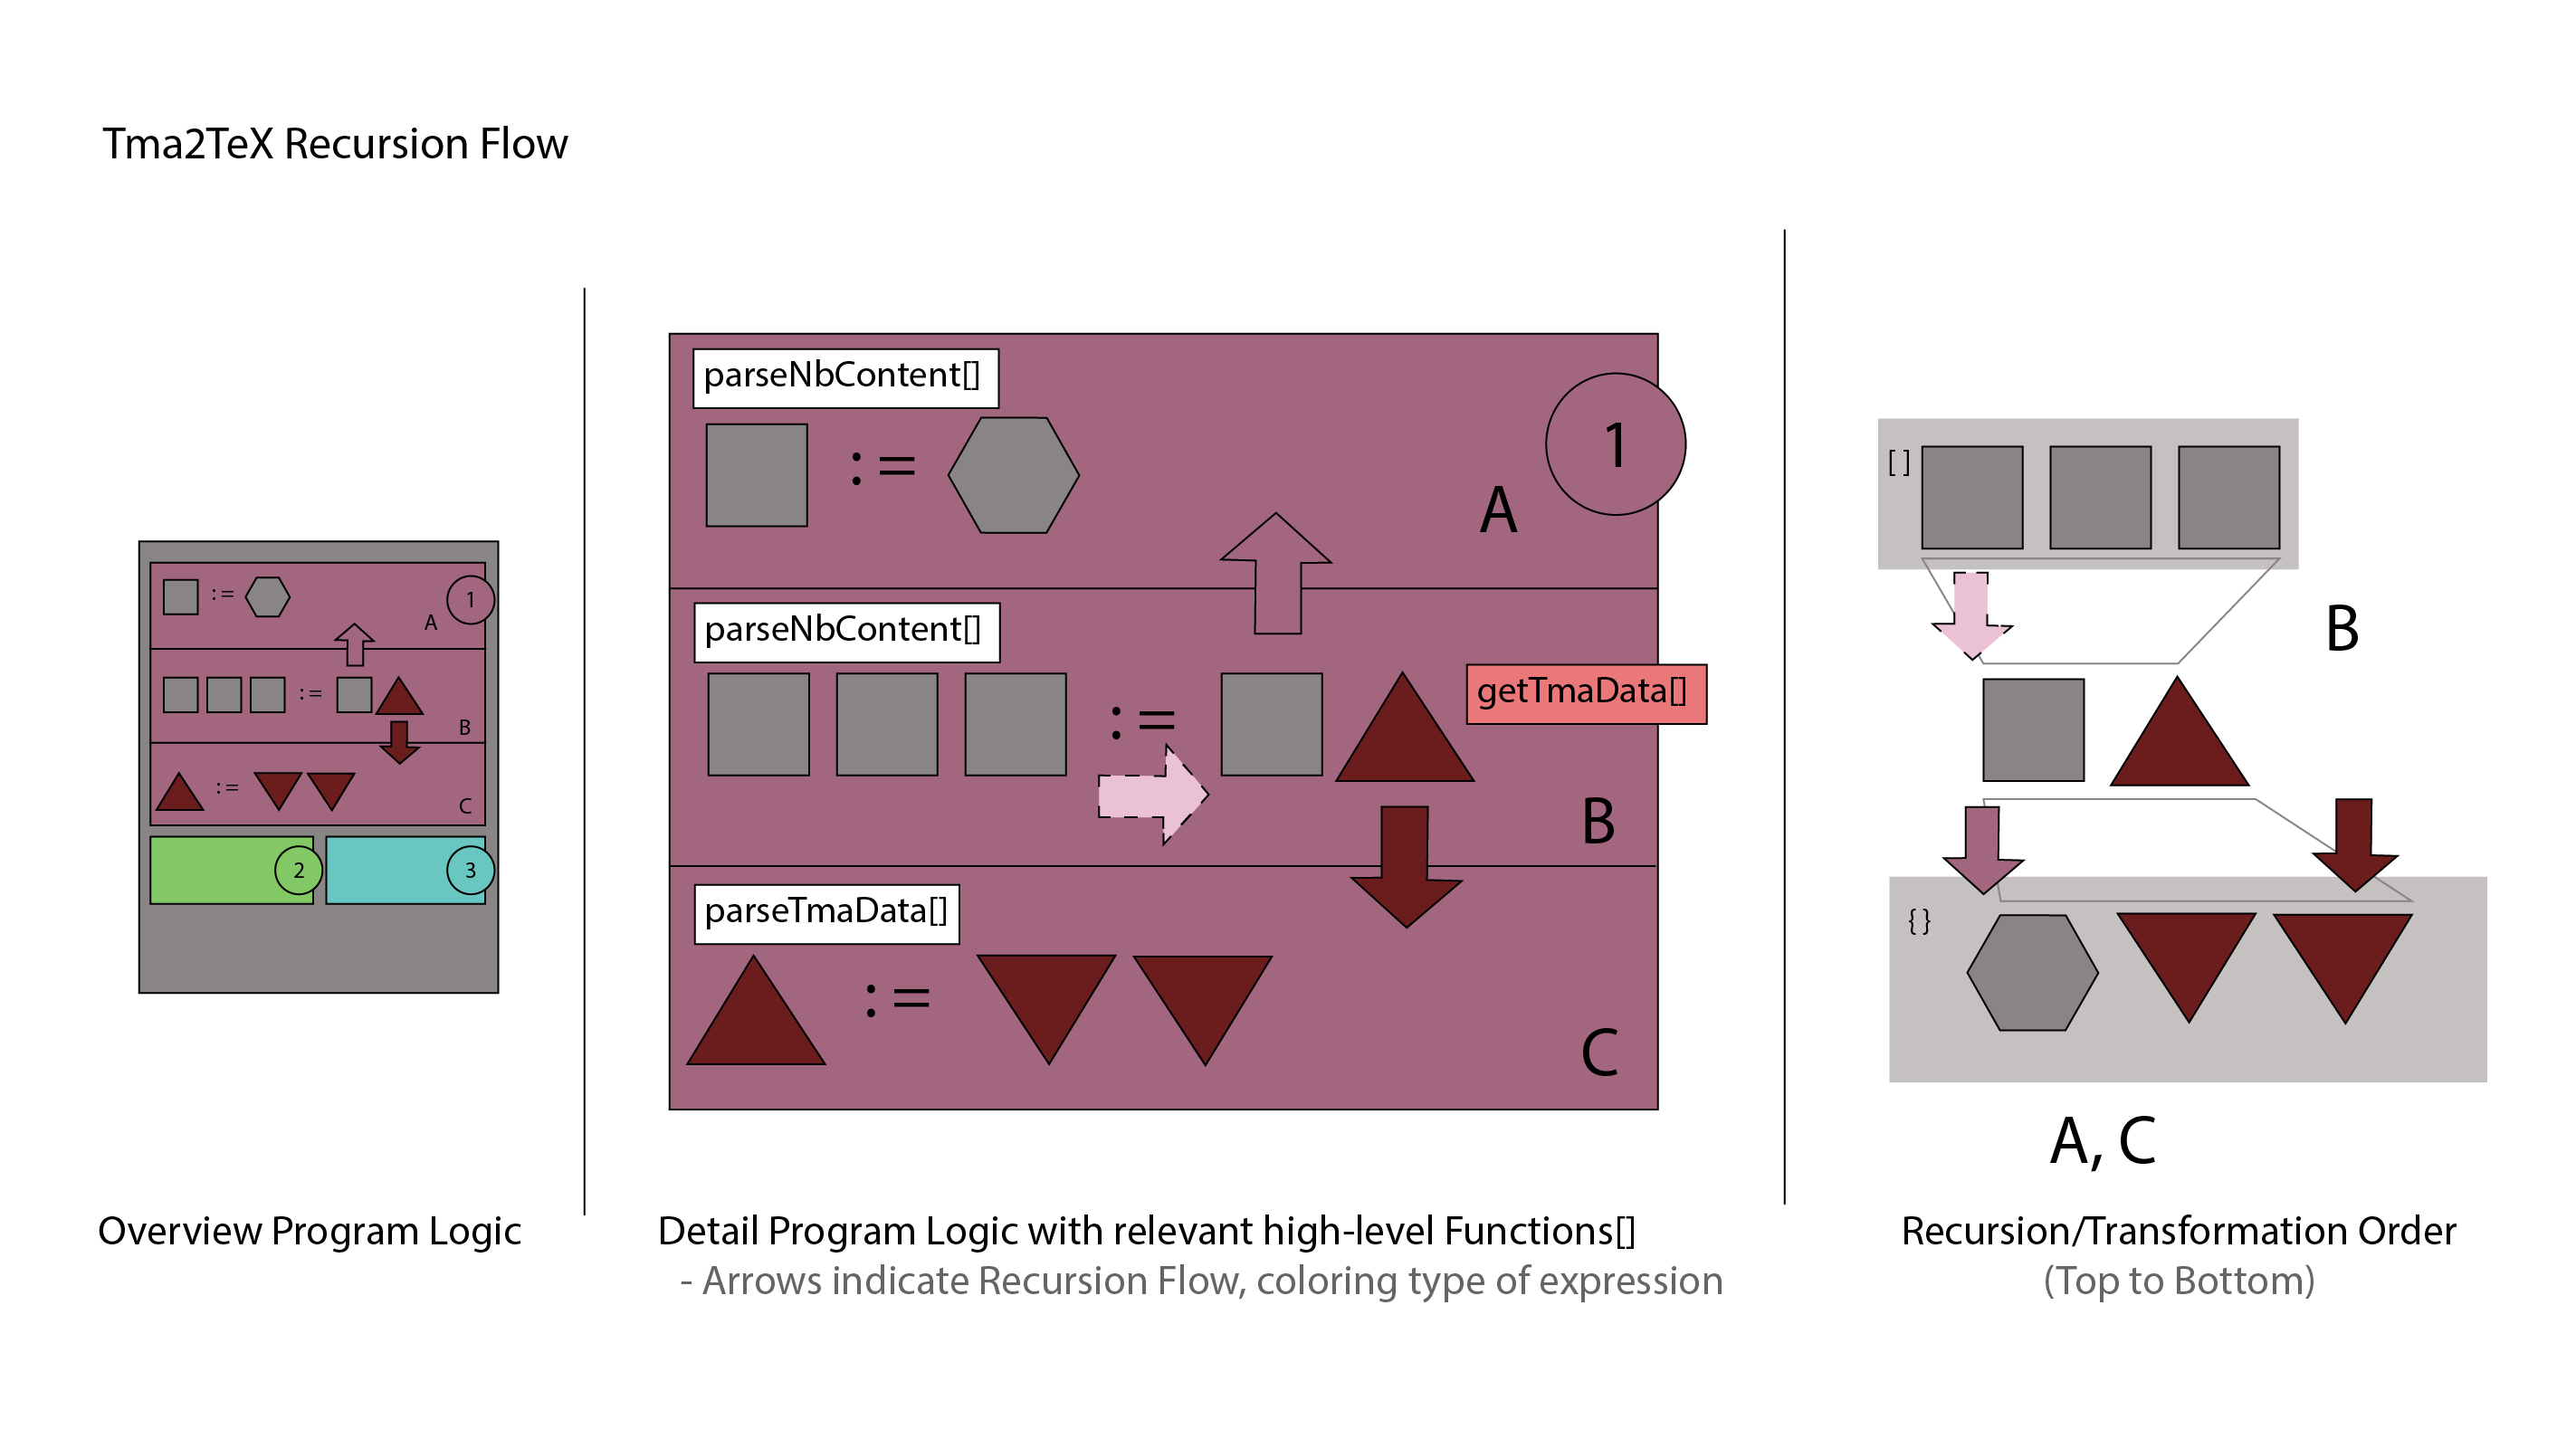
\includegraphics[scale=.35]{images/concept/Tma2Tex-Recursion-Flow-01.png}
    \caption{}
    \label{fig:high-level}
\end{figure}

Section \ref{pattern-matching-implementation} in the following chapter elaborates on the specificity rules crucial to the call order. Recursion is simple to see at this point: by adding a call to the same function on the right hand side of the rule, the rule becomes recursive. The core idea of this implementation is the fashioning of many rules that are applied according to the relevant Theorema Notebook pattern, called recursively and descended in the sense that we move from outer expression to inner-most. Indeed, we start from calling the relevant function, parseNotebookContent in the form \lstinline+parseNotebookContent[Notebook[l_List, ___]]+, that is, on the entire Notebook expression that represents a Mathematica notebook.

The same idea is applied twice, to two sets of patterns: once for general text and WL notebook expression syntax, and once for the more specific syntax specified by the Theorema Language. Hence it makes sense to speak of a double-recursion, or a double-descent, in this implementation. Theorema Language is rendered distinctively in the final \LaTeX/PDF output, to mark this distinction outwardly.

\subsection{Pattern Matching to Realize \LaTeX-Transformation of the Theorema Language Data Structure}

This subsection expands on the notion of the horizontal program dimension, after the live version of the current Theorema formula under consideration (being parsed) has been obtained, via getTmaData[]: now the goal is to generate a TeX-snippet like \verb| \IffTM{ \AndTM{ \ForallTM{ ...| with appropriate closing brackets from a formula like \verb|Theorema`Language`Iff$TM[ Theorema`Language`And$TM[ Theorema`Language`Forall$TM[ ...|. The easy suffix "TM" is chosen for the \LaTeX output, the "\$TM" visible in the Theorema Language code is the original way of keeping separate contexts. In this way Theorema may specify its own "Iff", "And", "Forall" etc., both in notebooks and the \LaTeX result of this project.

Roughly, there is a Predicate Logic distinction between operator symbols known to the language, marked by the word "Language" in the symbol name context, and knowledge outside of the language, functions and predicates with the word "Knowledge" in their context path. \cite{wolfram_research_inc_contextwolfram_2024} The parsing needs to result in square brackets for the "Knowledge"-symbols, and macro-syntax curly braces for the "Language"-symbols, with appropriate parameter placement. These macros, or commands, are then fully defined inside the \LaTeX-template file.

\section{Extensibility in Both \LaTeX and Wolfram Language}

\subsection{A Note on Evaluation Criteria and Stability}

The execution of the idea can be evaluated in terms of two core criteria. First, stability is a key criterion for this work and actually bases on generality of the patterns selected: WL and Theorema expression patters that will stand the test of time need to be selected at the development stage, and testing must include a diverse current range of Theorema notebooks. 

\subsection{WL-Messages and -Tests: Software Design Goals}

WL provides modern engineering-oriented functionality for both tests and error-handling, in the form of messages \cite{wolfram_research_inc_messagewolfram_2024} - the mechanism is part of this package such as in the case the file has not been loaded completely to provide the required formula data, see Figure \ref{fig:message-demo}.

\begin{figure}[h]
    \centering
    \includegraphics[scale=.8]{images/concept/Tma2Tex-Message-Demo.png}
    \caption{The basic idea is that every message has a definite name, of the form symbol::tag. \cite{wolfram_research_inc_textual_2024}}
    \label{fig:message-demo}
\end{figure}

Testing will make up a large part of Chapter \ref{cha:Closing}.

\subsection{Extensibility}

Extensibility at both the WL and \LaTeX levels is the other priority, with the understanding that Theorema Language might change, Wolfram Language might be updated, and additional \LaTeX commands or alternative rendering imperatives might be required.

The main extension points go as follows, where the sectioning of the code follows the final version submitted with this thesis for easier finding of the relevant code. At the WL-level:

\begin{itemize}
    \item \bold{Package Parts 1.B and 1.C}, where B covers the first recursive descent through the overall notebook structure and C the second descent into the Theorema-formula:
    
    \item \bold{formatTmaData} (1.C.3): wrapper function around the Formula-\LaTeX-output that maybe used for string replacements, for instance, at the level of the formula-\LaTeX snippets.
    \item \bold{Client-Functionality} (Part 3): both top level functions convertToLatexDoc and convertToLatexAndPdfDocs may be edited easily to suit the needs of higher-level project, while more rigid configuration details are hidden away in Part 2, especially as concerns filehandling details.
    \item \bold{Overall Package}: This project was developed as a package \"tma2tex\" but the code Parts 1 - 3 can easily be moved to another package, as long as Theorema, the overall package, is in some way available, and the global variables \lstinline+Tma2tex`\$resDir+ and \lstinline+Tma2tex`\$tmaData+ are readied.
\end{itemize}

The main extension procedure on the level of \LaTeX is to add macro-definitions in the template provided in \lstinline+Tma2tex`\$resDir+, in a file called \lstinline+tmaTemplate.tex+ in the default configuration. A sample set of macros is provided for reference in \lstinline+sampleTemplateMacros.tex+.

%\subsection{Ease of Use/Setup}